\section{Published-score scale context}
\begin{table*}[t]
\centering\footnotesize
\caption{\textbf{Published margins give scale, not paired significance.} Author-reported FID and its reported 95\% mean margin, beside our signed same-output raw$-C$ gap. Original five rows use HumanML3D; other datasets are labeled. Samples, readers, checkpoints and conditioning differ. MDM50/DiP use corrected author results; T2M uses estimated length. DiP is prefix-conditioned. These numbers do not test our gap against a published uncertainty or establish leaderboard reproduction.}\label{tab:publishedscale}
\begin{tabular}{@{}lrr@{}}\toprule
Method/dataset/setting&Published FID&Our raw$-C$\\\midrule
MDM50, corrected release~\cite{tevet2023}&$0.489\pm0.047$&+0.0046\\
MLD~\cite{mld2023}&$0.473\pm0.013$&-0.0038\\
MotionLCM, one step~\cite{motionlcm2024}&$0.467\pm0.012$&-0.0315\\
T2M-GPT, $\tau\sim U[0,1]$~\cite{t2mgpt2023}&$0.141\pm0.005$&+0.0340\\
T2M, estimated length~\cite{guo2022}&$1.087\pm0.021$&+0.0464\\
MoMask / HumanML~\cite{momask2024}&$0.045\pm0.002$&+0.0033\\
DiP / HumanML, corrected release~\cite{closd2025}&$0.228\pm0.027$&+0.0015\\
MotionDiffuse / HumanML, preprint~\cite{motiondiffuse2024}&$0.630\pm0.001$&-0.0041\\
MoMask / KIT, final table~\cite{momask2024}&$0.204\pm0.011$&-0.0137\\
MotionDiffuse / KIT, preprint~\cite{motiondiffuse2024}&$1.954\pm0.062$&-0.0364\\
\bottomrule\end{tabular}\end{table*}

Published FID margins contextualize the absolute representation changes (\cref{tab:publishedscale}). They estimate uncertainty of different means under different protocols; they are not uncertainties of our paired gaps. No cross-paper significance test follows. The T2M-GPT uniform-corruption, MLD and one-step MotionLCM rows come from their respective papers. T2M uses its estimated-length result, $1.087\pm0.021$; the separate real-length row is $1.067\pm0.002$.

MoMask uses the final CVPR table, including KIT $0.204\pm0.011$ rather than the abstract's 0.228. MotionDiffuse scale values come from the 2022 author preprint associated with its public release (\url{https://arxiv.org/abs/2208.15001}); the bibliography cites its journal publication. DiP's corrected author table reports $0.228\pm0.027$. Our checkpoint and prefix setting are recorded separately. These numerical sources provide scale context, not proof that our inference settings reproduce each published experiment.

MDM50's corrected $0.489\pm0.047$ comes from the authors' maintained results rather than the original 1000-step paper row. The pinned release includes the result at \url{https://github.com/GuyTevet/motion-diffusion-model/blob/ef8edce6a53c6ab19e53b4d4dcf15bc0bc60a778/assets/fixed_results.tex}; its revision and fingerprint are recorded with the artifacts. We do not mix the old paper margin with this 50-step checkpoint or interpret the published score as a reproduction target for our capped-output audit.

\section{Additional public releases and native KIT-ML}
\begin{table*}[t]
\centering\footnotesize
\caption{\textbf{Additional releases and KIT.} All 20 draws, own native evaluator normalization, same-output raw/C. Intervals for raw$-C$ adjust ten FID/R1 comparisons. HumanML MoMask uses 4,640 outputs; MotionDiffuse/DiP use 1,024 with full reference. KIT uses 704 outputs/reference. DiP is prefix-conditioned; published-score reproduction is not claimed.}\label{tab:additionalfull}
\begin{tabular}{@{}lrrrrrr@{}}\toprule
Data/release&Raw FID&$C$ FID&FID gap interval&Raw R1&$C$ R1&R1 gap interval\\\midrule
humanml/MoMask&0.0677&0.0644&$[+0.00279,+0.00382]$&0.4632&0.4626&$[-0.0010,+0.0023]$\\
humanml/DiP (prefix)&0.3665&0.3650&$[+0.00004,+0.00303]$&0.4518&0.4518&$[-0.0022,+0.0023]$\\
humanml/MotionDiffuse&0.9766&0.9807&$[-0.00737,-0.00076]$&0.4277&0.4273&$[-0.0018,+0.0026]$\\
kit/MoMask&0.3512&0.3649&$[-0.02473,-0.00270]$&0.4175&0.4181&$[-0.0070,+0.0057]$\\
kit/MotionDiffuse&1.7794&1.8159&$[-0.04282,-0.03002]$&0.4125&0.4116&$[-0.0017,+0.0036]$\\
\bottomrule\end{tabular}\end{table*}

MoMask~\cite{momask2024} uses the released residual VQ model, latest masked-transformer checkpoint and best-FID residual checkpoint. Inference uses 18 mask steps, CFG 4, temperature 1, top-k threshold 0.9, no Gumbel sampling, then residual CFG 5. The native decoder and its normalization remain unchanged. Prescribed durations are supplied; future source poses are not inputs. Both HumanML3D and native KIT use the full eligible test cohorts after dropping the incomplete 32-item batch, with 20 draws.

MotionDiffuse~\cite{motiondiffuse2024} uses the author encoder and normalization, native linear 1000-step DDPM, epsilon prediction and fixed-small variance. Prescribed durations follow the native 40-frame HumanML/24-frame KIT minimum. An elementwise-equivalent device mask removes the upstream Python frame loop; mask/full-forward equality is checked. Compilation retains all native layers, weights and float32 operations with TF32 disabled. Operator fusion changes rounding slightly, so compiled/eager parity residuals are reported, rather than claiming bit identity. Inference batches are 128; HumanML outputs are capped at 1,024 with a full reference, and KIT uses the full 704-output cohort. These are paired consistency audits, not an exact reproduction of published scores.

DiP~\cite{closd2025} uses the no-target author checkpoint at 200,000 steps with EMA, DistilBERT and native autoregressive sampling: context 20, prediction 40, 10 diffusion steps, CFG 7.5. The first 20 frames of each saved cropped source motion initialize its prefix, excluded from the generated output. No future source frames are passed. This prefix-conditioned setting differs from text-only generation and is not a claim that DiP constitutes an unrelated MDM architecture. Twenty 1,024-output draws use full real references.

Native KIT~\cite{kit2016} uses the official processed MMM archive and its 251-feature T2M evaluator. Its 20 local 6D rotations occupy 64:184; the evaluator excludes the final four contact channels. Its real test reference and outputs contain 704 native entries per draw, including segment annotations. The separate TMR KIT AMASS model consumes 263 features and is incompatible with this archive. It is not substituted or padded to accept 251 features.

All raw/canonical pairs share emitted arrays, captions, masks, candidate groups and reference. Additional-release uncertainty is analyzed jointly within its comparison family; absolute signed differences remain separate from published mean margins. Sources, archive hashes, native-component checks and complete output arrays accompany the artifacts. Native KIT coordinates differ in scale from HumanML meters, so its FK residuals are reported in native units and relative to body height; KIT inputs are never rescaled before evaluation.

\section{Independent Transformer evaluator}
\begin{table*}[t]
\centering\footnotesize
\caption{\textbf{Different architecture, modest natural dependence.} Native TMR cosine/sample-mean inference on compatible existing cohorts; 20 draws, family12 intervals for raw$-C$. This is not the full official annotation/filter protocol.}\label{tab:tmrnatural}
\begin{tabular}{@{}lrrrrrr@{}}\toprule
Source&Raw R1&$C$ R1&R1 gap interval&Raw cosine&$C$ cosine&Cosine gap interval\\\midrule
Real&0.6784&0.6784&$[+0.0000,+0.0000]$&0.5245&0.5245&$[-0.00000,+0.00000]$\\
MDM50&0.5578&0.5571&$[-0.0015,+0.0029]$&0.4296&0.4299&$[-0.00040,-0.00016]$\\
MLD&0.5848&0.5841&$[-0.0005,+0.0019]$&0.4527&0.4526&$[+0.00002,+0.00024]$\\
MotionLCM-v1&0.6785&0.6757&$[+0.0013,+0.0043]$&0.5035&0.5024&$[+0.00098,+0.00132]$\\
T2M-GPT&0.6703&0.6698&$[-0.0006,+0.0017]$&0.5335&0.5331&$[+0.00035,+0.00057]$\\
T2M&0.5626&0.5611&$[+0.0003,+0.0028]$&0.4331&0.4311&$[+0.00182,+0.00208]$\\
\bottomrule\end{tabular}\end{table*}

TMR~\cite{tmr2023} uses author ACTOR motion/text encoders with six Transformer layers and 256 latent dimensions. Motion input has 263 features and the author mean/std with epsilon $10^{-12}$. Frozen DistilBERT supplies 768-dimensional token embeddings. Native deterministic inference takes the VAE mean token; similarity is normalized cosine. Author weights are loaded strictly and the archive's supplied MD5 is verified.

The natural audit reuses the original five public generators and real-motion cohorts across 20 draws. Raw/canonical, fixed $\pm 0.1/\pm 0.35$ and random 0.35 are all scored. Random fields use seed 42 plus global clip index, independently per record, differing from the T2M fixed-control field. Twelve paired R1/cosine endpoints use family-adjusted$t_{19}$ intervals. We retain the compatible T2M-feature cohorts, candidate batches of 32 and their annotations rather than reproduce TMR's full AMASS annotation/semantic-filter protocol. In particular, no semantic-neighbor filter or full-gallery retrieval score is claimed.

Natural R1 differences are small: MotionLCM and T2M have positive intervals; other generated-source intervals include zero. Matched cosine detects additional changes but is a separate endpoint. Real R1 is identical before/after canonicalization. Saved scores, native forward outputs and batch/serial motion embeddings are independently checked. DistilBERT padding/batch changes cause float32 text differences below $4.7\times 10^{-5}$; matching the producer's 64-caption cache batches reproduces saved vectors. This arithmetic diagnostic is not a new evaluation protocol.

\begin{table*}[t]
\centering\small
\caption{\textbf{All TMR attack controls on 1,024 clips/source.} Wrong targets are a circular caption shift. The generic attack matches the rotation-fiber attack\'s per-clip standardized L2 radius while changing continuous features. Canonical source and attacked R1 agree within each source; raw/canonical source scores may differ.}\label{tab:tmrattackfull}
\begin{tabular}{@{}llrrrr@{}}\toprule
Source&Condition&Actual R1&Wrong R1&$\C$ actual R1&Actual cosine\\\midrule
Real&original&0.688&---&0.688&0.524\\
Real&actual target&1.000&0.000&0.688&0.944\\
Real&wrong target&0.015&0.968&0.688&0.140\\
Real&canonical gradient&0.688&0.010&0.688&0.524\\
Real&generic L2&1.000&---&1.000&0.991\\
MDM&original&0.578&---&0.580&0.426\\
MDM&actual target&0.993&0.000&0.580&0.920\\
MDM&wrong target&0.022&0.946&0.580&0.146\\
MDM&canonical gradient&0.578&0.017&0.580&0.426\\
MDM&generic L2&1.000&---&1.000&0.991\\
\bottomrule\end{tabular}\end{table*}

Capability tests use all 1,024 fixed clips per source of the fixed caption-targeted cohort, with real and MDM sources, 80 Adam steps, learning rate 0.1, bound 0.35 and final iterate. The reader remains frozen. Targets are actual or circularly shifted captions; the canonical-gradient control differentiates through canonical input. Every target/canonical endpoint is included. The source clips now match the T2M cohort; native cosine similarity and candidate permutations still differ, preventing an across-architecture accuracy ranking.

Actual-target R1 changes 0.688 to 1.000 on real motion and 0.578 to 0.993 on MDM; wrong targets also redirect retrieval while actual-target agreement decreases. Canonical embeddings change by at most $6.7\times 10^{-6}$. Canonical MDM R1 is 0.580 both before and after recoding, distinct from source raw R1 0.578. Independent native checks cover 6,144 clip pairs and 48 FK samples: maximum angle $2.0\times 10^{-5}$ degrees, maximum FK displacement $9.6\times 10^{-7}$ m, bitwise protected channels and unchanged padding.

\paragraph{Generic adversary at matched L2.}
For each clip, we measure the actual-target rotation-fiber attack's L2 radius in TMR-normalized units over valid frames. A generic 80-step Adam attack changes all 259 continuous features, keeps contacts/padding fixed and projects onto that per-clip radius after every update. It reaches perfect retrieval and remains effective under canonicalization. Mean RIC position changes are 0.810 m real/0.899 m MDM, and mean rotation changes are 25.2/25.7 degrees. The features can be physically inconsistent across blocks. This comparison does not claim a smallest physical adversary; it demonstrates the distinct guarantee of zero physical change inside the rotation fiber. Verified radius excess is at most $3.1\times 10^{-5}$ normalized units.

\section{Physical angular sensitivity}
\begin{table}[t]
\centering\footnotesize
\caption{\textbf{Coherent physical calibration.} Means across 20 full real cohorts; paired coherent zero reference, common four-frame crop. Original-to-zero cost is explicit. Doses are local nonroot rotation angles, with fixed-per-clip or independent-per-frame axes. All recodings preserve that reconstructed movement.}\label{tab:physicalcal}
\begin{tabular}{@{}lrrr@{}}\toprule
Condition&FID&R1&MM-dist.\\\midrule
Original vs reconstruction&0.02006&0.4510&3.2545\\
Coherent zero&3.353e-10&0.4474&3.2707\\
$C$ of coherent zero&1.74e-10&0.4474&3.2707\\
Fixed recoding $+0.1$&0.05898&0.4461&3.2749\\
Fixed recoding $-0.1$&0.08278&0.4386&3.3222\\
Fixed recoding $+0.35$&1.972&0.3900&3.7303\\
Fixed recoding $-0.35$&3.574&0.3565&3.9646\\
Random recoding $0.35$&0.02445&0.4418&3.2952\\
Fixed axes, $0.1^\circ$&3.661e-07&0.4474&3.2707\\
Fixed axes, $0.3^\circ$&3.476e-06&0.4474&3.2707\\
Fixed axes, $1^\circ$&6.385e-05&0.4475&3.2707\\
Fixed axes, $3^\circ$&0.002647&0.4468&3.2723\\
Fixed axes, $10^\circ$&0.2996&0.4268&3.3625\\
Fixed axes, $30^\circ$&14.44&0.2432&5.4553\\
Framewise axes, $0.1^\circ$&1.624e-05&0.4474&3.2708\\
Framewise axes, $0.3^\circ$&0.001198&0.4485&3.2718\\
Framewise axes, $1^\circ$&0.3502&0.4408&3.3283\\
Framewise axes, $3^\circ$&10.24&0.3621&4.3791\\
Framewise axes, $10^\circ$&38.98&0.2186&6.5188\\
Framewise axes, $30^\circ$&75.17&0.0970&8.7587\\
\bottomrule\end{tabular}\end{table}

We perturb the 21 nonroot rotations using local SO(3) angles 0.1/0.3/1/3/10/30 degrees. Gaussian random axes are normalized per joint, either fixed throughout a clip or independently drawn at each frame. Axes share seeds across angle doses, with deterministic per-record indexing, and both noise modes use all 20 saved real test cohorts. No angle or clip is selected by a score.

Forward kinematics uses the native skeleton and each clip's initial bone lengths. Root trajectory stays fixed. Rotations, RIC positions, root-local joint velocities and native foot-contact predicates are updated together. A common four-frame crop supplies next-frame positions for velocities. The reference is the paired coherent zero-angle reconstruction; its FID-zero baseline is therefore by construction. Original-to-reconstruction FID is 0.0201 and R1 changes 0.4510$\to$0.4474, so reconstruction cost is not hidden.

On this same coherent reference, fixed $+0.35/-0.35$ recodings give FID 1.972/3.574 with zero physical change. These levels lie between the measured 1- and 3-degree frame-independent doses, but between 10 and 30 degrees with temporally fixed axes. These are brackets on the measured curves, not a universal degree equivalence, perceptual claim or result of new interpolated-dose experiments. Full FID/R1/MM curves, small/random recodings and nominal$t_{19}$ mean intervals are reported.

Independent checks verify 240 physical clip cases, native SO(3) angles, RIC/FK agreement, recomputed local velocities/contacts, fixed roots and padding. Saved metric endpoints are recomputed against their exact references. The reconstruction follows native geometry conventions; it is not a licensed SMPL mesh or human-quality calibration.

\section{Caption-blind cross-generator and cross-reader transfer}
\begin{figure*}[t]\centering
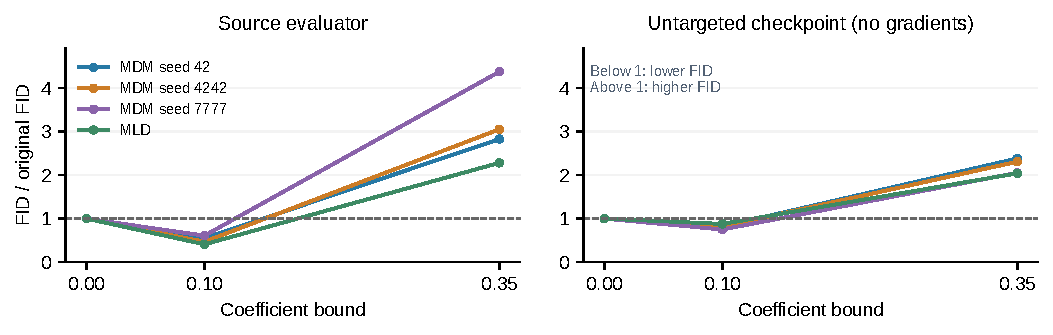
\includegraphics[width=\textwidth]{figures/blind_checkpoint_transfer.pdf}
\caption{\textbf{Caption-blind attacks transfer without destination gradients.} Every attacked output is sealed before reference scoring. Lines show FID divided by the same reader/cohort's original FID, for all tested bounds: source T2M weights on the left and another official checkpoint of the same architecture on the right. MLD supplies another generator; the three MDM cohorts overlap in source groups and are repetitions, not independent clip samples. Bound 0.1 helps every cohort; 0.35 harms every cohort.}\label{fig:blindtransfer}\end{figure*}

\begin{table*}[t]
\centering\footnotesize
\caption{\textbf{Sealed blind attacks on both generators and checkpoints.} FID for 960 outputs/cohort; both budgets, canonical-gradient and random controls. Destination checkpoint supplies no gradients. MDM groups overlap, so there is no pooled independent-clip interval.}\label{tab:blindtransfer}
\begin{tabular}{@{}llrrrrr@{}}\toprule
Cohort&Reader&Original&Bound0.1&Bound0.35&$C$ grad.&Random\\\midrule
mdm42&Source&0.3839&0.2099&1.0850&0.3839&0.3526\\
mdm42&Transfer&0.4083&0.3338&0.9718&0.4083&0.4965\\
mdm4242&Source&0.3762&0.1761&1.1477&0.3762&0.3231\\
mdm4242&Transfer&0.3710&0.3030&0.8555&0.3710&0.3790\\
mdm7777&Source&0.3268&0.1987&1.4292&0.3268&0.3011\\
mdm7777&Transfer&0.3793&0.2839&0.7786&0.3793&0.4319\\
mld&Source&0.7064&0.2886&1.6108&0.7064&0.6698\\
mld&Transfer&0.6594&0.5786&1.3452&0.6594&0.8104\\
\bottomrule\end{tabular}\end{table*}

MLD reuses the first 960 eligible outputs from native repetition 0 after excluding every original target-aware test source/mirror group. Selection is based on source identity, not scores. Segment names map to their underlying source before exclusion. The reference motion/captions are sealed separately; training targets, budgets 0.1/0.35 and 80-step final-iterate Adam match the MDM protocol. Native output durations, captions and reference crops remain paired. This is a new generator source but not a globally untouched test split.

The MLD source-reader FID changes 0.7064$\to$0.2886 at 0.1 and worsens to 1.6108 at 0.35. Canonical-gradient controls remain at baseline. Native reconstruction verifies 5,760 equivalent pairs and 48 FK samples; position/contact/velocity features stay bitwise unchanged. Maximum FK difference is$6.0\times 10^{-7}$ m.

All four sealed cohorts are then scored by the untargeted official T2M-GPT checkpoint, with the same architecture and normalization but distinct weights. No destination gradients, refitting or new target moments are used. At bound 0.1, MDM FID reductions are 18.2/18.3/25.1\%; MLD reduces 12.3\%. The larger budget worsens every cohort. Canonicalization closes the channel in the destination reader as well. These transfer changes are descriptive, not an independent-generator or population CI.

The two further MDM cohorts have 769 and 761 unique source groups; their intersection is 493. Their overlap with the first blind cohort is 494/496. Shared training targets and source overlap are disclosed; no pooled independent-clip interval is reported. FID changes are evaluator effects at identical represented movement, not improved generator quality.

\section{Canonical real-data sanity checks and portable implementation}
\begin{table}[t]
\centering\footnotesize
\caption{\textbf{Sanity check on already canonical real motion.} Twenty paired native draws. HumanML primary/secondary share an architecture; TMR differs. KIT uses its 251-feature evaluator. R1 equality is expected for already canonical rotations and does not establish accuracy cost on noncanonical inputs.}\label{tab:defensecost}
\begin{tabular}{@{}lrrr@{}}\toprule
Data/reader&Raw R1&$C$ R1&$C-$raw\\\midrule
HumanML primary&0.45275&0.45275&+0.00000\\
HumanML secondary&0.51222&0.51222&+0.00000\\
HumanML TMR&0.67842&0.67842&+0.00000\\
KIT primary&0.42443&0.42443&+0.00000\\
\bottomrule\end{tabular}\end{table}

Across 20 paired native draws, HumanML R1 raw/canonical is 0.45275/0.45275 for the primary T2M reader, 0.51222/0.51222 for the secondary reader and 0.67842/0.67842 for TMR. KIT real-motion R1 is 0.42443 in both paths. The paired R1 differences are exactly zero in these observations. Small floatingpoint embedding differences are measured separately. These real-motion rotations are already canonical. The unchanged retrieval therefore checks numerical implementation; it is not empirical evidence of a cost-free defense on noncanonical inputs. Matched sign-language reader adaptation is reported separately.

A portable NumPy implementation canonicalizes the two consecutive 3-vectors before evaluator normalization, validates the nondegenerate domain and preserves every nonrotation channel and padded frame bitwise. Tests cover arbitrary positive scale/shear, idempotence, orthogonality, both native schemas and invalid rotations. The accompanying evaluation contract specifies converter convention, input normalization, masking and reader-fitting/inference agreement. It closes only the 6D fiber; generic physical or cross-feature attacks remain possible.
